\documentclass{article}

%\usepackage[dvipsnames]{xcolor}
\usepackage{titletoc}
\usepackage[page,header]{appendix}
\usepackage{tcolorbox}
% Recommended, but optional, packages for figures and better typesetting:
\usepackage{geometry}
\geometry{a4paper, scale=0.8}
\usepackage{microtype}
\usepackage{graphicx}
\usepackage{subfigure}
\usepackage{booktabs} % for professional tables
\usepackage{algorithm}
\usepackage{algorithmic}
% hyperref makes hyperlinks in the resulting PDF.
% If your build breaks (sometimes temporarily if a hyperlink spans a page)
% please comment out the following usepackage line and replace
% \usepackage{icml2024} with \usepackage[nohyperref]{icml2024} above.
%\usepackage{hyperref}
\usepackage{hyperref}
%\hypersetup{hidelinks}

% Attempt to make hyperref and algorithmic work together better:
\newcommand{\theHalgorithm}{\arabic{algorithm}}

% Use the following line for the initial blind version submitted for review:
% \usepackage{icml2024}

% If accepted, instead use the following line for the camera-ready submission:
% \usepackage[accepted]{icml2024}

% For theorems and such
\usepackage{amsmath}
\usepackage{amssymb}
\usepackage{mathtools}
\usepackage{amsthm}

% if you use cleveref..
% \usepackage[capitalize,noabbrev]{cleveref}

%%%%%%%%%%%%%%%%%%%%%%%%%%%%%%%%
% THEOREMS
%%%%%%%%%%%%%%%%%%%%%%%%%%%%%%%%
\theoremstyle{plain}
\newtheorem{theorem}{Theorem}[section]
\newtheorem{proposition}[theorem]{Proposition}
\newtheorem{lemma}[theorem]{Lemma}
\newtheorem{corollary}[theorem]{Corollary}
\theoremstyle{definition}
\newtheorem{definition}[theorem]{Definition}
\newtheorem{assumption}[theorem]{Assumption}
\theoremstyle{remark}
\newtheorem{remark}[theorem]{Remark}
\usepackage{comment}
\newtheorem{observation}[theorem]{Observation}
\newtheorem{fact}[theorem]{Fact}

% Todonotes is useful during development; simply uncomment the next line
%    and comment out the line below the next line to turn off comments
%\usepackage[disable,textsize=tiny]{todonotes}
\usepackage[textsize=tiny]{todonotes}
\usepackage{pdfcomment}
\newcommand{\commentontext}[2]{\colorbox{yellow!60}{#1}\pdfcomment[color={0.234 0.867 0.211},hoffset=-6pt,voffset=10pt,opacity=0.5]{#2}}
\newcommand{\commentatside}[1]{\pdfcomment[color={0.045 0.278 0.643},icon=Note]{#1}}
\usepackage{moreenum}
\usepackage{mathtools}
\usepackage{url}
\usepackage{bm}
\usepackage{enumitem}
\usepackage{graphicx}
\usepackage{listings}
\usepackage{color}
\usepackage{subcaption}
\usepackage{booktabs} % toprule
\usepackage[mathcal]{eucal}
\usepackage{tikz}
\usepackage{dsfont}
\usepackage{bbm}
\usepackage{cancel}
\usepackage{physics}
\usepackage{authblk}
\usepackage{mathrsfs}
\usepackage[justification=centering]{caption} 
\usepackage{graphicx}
\usepackage{float}
\usepackage[export]{adjustbox} 
\usepackage{caption}
\usepackage{subcaption}
\usepackage{float}
\usepackage[export]{adjustbox} 
\usepackage{caption}
\usepackage{subcaption}
\renewcommand\contentsname{Content}


\usepackage[marginal]{footmisc}

% add these two lines to your long preamble



% Optional math commands from https://github.com/goodfeli/dlbook_notation.






\renewcommand{\thefootnote}{\fnsymbol{footnote}}
\renewcommand*{\thefootnote}{\arabic{footnote}}



\definecolor{ForestGreen}{RGB}{34,139,34}
\newcommand{\com}[1]{\textcolor{green}{ #1}}
\newcommand{\revise}[1]{\textcolor{orange}{#1}}
\newcommand{\algcomshort}[1]{\textcolor{blue}{{\hfill $\triangleright$ { #1}}}}
\newcommand{\algcom}[1]{\textcolor{blue}{ #1}}
%%%%%%%%%%%%%%%%%%%%%%%%%%%%%%%%%%%%%%%%%%%%%%%%%%%%%%%%%%%%%%%%%
%%%%%%%%%%%%%%%%%%%%  font color setting  %%%%%%%%%%%%%%%%%%%%%%%
%%%%%%%%%%%%%%%%%%%%%%%%%%%%%%%%%%%%%%%%%%%%%%%%%%%%%%%%%%%%%%%%%
\newcommand{\red}[1]{\textcolor{red}{#1}}
\newcommand{\blue}[1]{\textcolor{blue}{#1}}
\newcommand{\green}[1]{\textcolor{ForestGreen}{#1}}
\newcommand{\purple}[1]{\textcolor{purple}{#1}}
\newcommand{\orange}[1]{\textcolor{orange}{#1}}
\newcommand{\pink}[1]{\textcolor{pink}{#1}}
\usepackage{hyperref}
\hypersetup{colorlinks,linkcolor={ForestGreen},citecolor={blue},urlcolor={blue}}
%%%%%%%%%%%%%%%%%%%%%%%%%%%%%%%%%%%%%%%%%%%%%%%%%%%%%%%%%%%%%%%%%
%%%%%%%%%%%%%%%%%%%%%%%%%%%%%%%%%%%%%%%%%%%%%%%%%%%%%%%%%%%%%%%%%



%%%%%%%%%%%%%%%%%%%%%%%%%%%%%%%%%%%%%%%%%%%%%%%%%%%%%%%%%%%%%%%%%
%%%%%%%%%%%%%%%%%%%%%% mathematical commands %%%%%%%%%%%%%%%%%%%%
%%%%%%%%%%%%%%%%%%%%%%%%%%%%%%%%%%%%%%%%%%%%%%%%%%%%%%%%%%%%%%%%%
\DeclareMathAlphabet{\mathcal}{OMS}{cmsy}{m}{n}
\SetMathAlphabet{\mathcal}{bold}{OMS}{cmsy}{b}{n}
\newcommand{\bigO}{\mathcal{O}}
\newcommand{\bigOmega}{\mathcal{O}}
\newcommand{\cT}{\mathcal{T}}
\newcommand{\cX}{\mathcal{X}}

\newcommand{\T}{\mathbb{T}}
\newcommand{\B}{\mathbf{B}}
\renewcommand{\O}{\mathbb{O}}
\newcommand{\Z}{\mathbb{Z}}
\newcommand{\R}{\mathbb{R}}
\newcommand{\lt}{\ensuremath <}
\newcommand{\gt}{\ensuremath >}

\newcommand{\D}{\mathscr{D}} 
\renewcommand{\r}{\boldsymbol{\rho}}
\newcommand{\p}{\mathbf{p}}
\newcommand{\BS}{\Delta(\mathscr{S})}  %Belief State
\newcommand{\E}{\mathbb{E}}
\renewcommand{\|}{\Bigg|}
\renewcommand{\[}{\left[}
\renewcommand{\]}{\right]}
\renewcommand{\(}{\left(}
\renewcommand{\)}{\right)}
\newcommand{\x}{\mathbf{x}}
\newcommand{\s}{\mathbf{s}}
\renewcommand{\a}{\mathbf{a}}
\newcommand{\m}{\mathbf{m}}
\newcommand{\n}{\mathbf{n}}
\newcommand{\e}{\mathbf{e}}
\renewcommand{\v}{\mathbf{v}}
\renewcommand{\u}{\mathbf{u}}
\renewcommand{\P}{\mathbb{P}}
\newcommand{\y}{\mathbf{y}}
\renewcommand{\H}{\mathbf{H}}
\newcommand{\Regret}{\text{Regret}}
\renewcommand{\wp}{\text{with probability at least $1-\delta$}}
\newcommand{\abbr}{\overset{abbr}{=}}
%spaces
\newcommand{\sS}{\mathscr{S}}
\newcommand{\sA}{\mathscr{A}} 
\newcommand{\sO}{\mathscr{O}} 
\newcommand{\sU}{\mathscr{U}}
\newcommand{\sF}[1]{\mathscr{F}_{#1}}
\newcommand{\sT}[1]{\mathcal{T}_{#1}} 
%random variables
\renewcommand{\S}{\mathbf{S}}
\newcommand{\A}{\mathbf{A}}
\renewcommand{\O}{\mathbf{O}} 
\newcommand{\F}{{\boldsymbol{F}}}
\newcommand{\f}{{f}}
\newcommand{\btau}{\boldsymbol{\tau}}

%matrices
\newcommand{\bT}{\mathbb{T}}
\newcommand{\bO}{\mathbb{O}}
\newcommand{\bM}{\mathbb{M}}
\newcommand{\bL}{\Lambda}
\newcommand{\K}{\mathcal{K}}
\renewcommand{\b}{{\vec{b}}}
%Shortcuts for operators
\DeclareMathOperator*{\argmax}{argmax}
\DeclareMathOperator*{\argmin}{argmin}
\newcommand{\Max}[1]{\underset{ #1 }{\max \ }}
\newcommand{\Min}[1]{\underset{ #1 }{\min \ }}
\newcommand{\Argmax}[1]{\underset{ #1 }{\argmax\ }}
\newcommand{\Argmin}[1]{\underset{ #1 }{\argmin\ }}
\newcommand{\sgn}{\text{sgn}}
\newcommand{\Pm}[1]{\mathbb{P}_{\mathcal{P}}\left\{ #1 \right\}}
%probability given the model
\renewcommand{\Pr}[1]{\mathbb{P}_{\mathcal{P}}^\pi\left\{ #1 \right\}} %probability given the model and the policy
\newcommand{\diag}[1]{\text{diag}\left(#1\right)}%diagonal matrix
\renewcommand{\over}[1]{\overset{#1}{=}}
\newcommand{\muu}[1]{\vec{\mu}_{#1}}
\newcommand{\V}{\mathsf{V}}
%sign function
\newcommand{\sign}[1]{\sgn{#1}}
%math symbols



\title{
Computer Vision and Image Analysis
\protect\\
Course Project Proposal
}

\author{
    Tonghe Zhang    \\
    Third-year Undergraduate Student From EE class 7\\
    Department of Electronic Engineering, Tsinghua University
    \texttt{zhang-th21@mails.tsinghua.edu.cn}\\
}

\date{\today}

\begin{document}
\maketitle



\section{Introduction}
This proposal draws the technical blueprint for the computer vision project, which aims to 
train a neural network to execute image segementation task 
on a human stenosis dataset. 

\section{Preliminary Experimental Results}
\paragraph*{Training}
We run the simplest algorithm provided with the project description and we keep the hyperparametes unchanged, which indicates that we will train the model for 10 epochs. In each epoch 250 training samples are used.
our model is trained on a single AMD A40 GPU. Empirically, running each epoch costs some 83 seconds. The loss curve in the entire training process is presented below:
\begin{figure}[H]
    \centering
    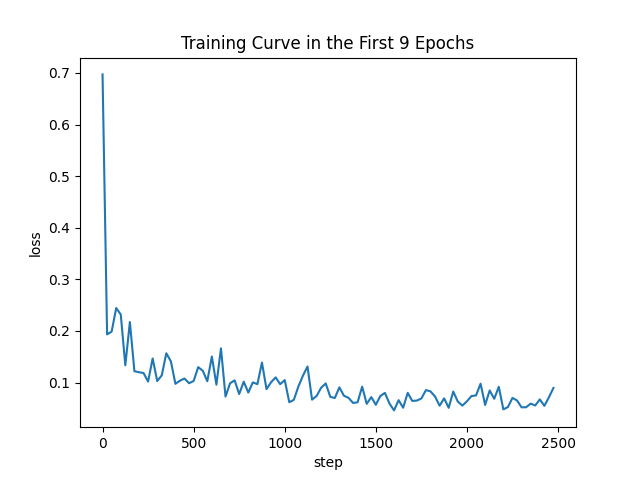
\includegraphics[width=0.65\textwidth,height=0.35\textwidth]{loss_curve.png}
\end{figure}
We can see that the loss curve goes down quickly. 

\paragraph*{Evaluation}
When evaluating the models saved in different epochs with the validation set, we obtain the following result:
\begin{figure}[H]
    \centering
    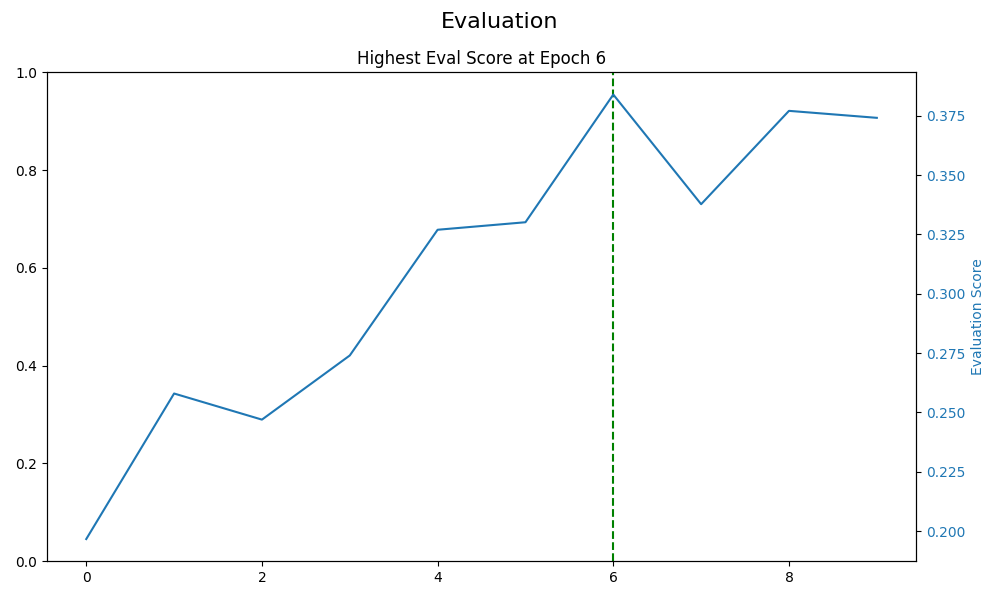
\includegraphics[width=0.65\textwidth,height=0.35\textwidth]{eval.png}
\end{figure}
which indicates that the best model in this simplest setting is 
obtained in epoch 6 and further training only causes the function approximator 
to overfit the training set. 

\paragraph*{Testing}
We test the trained model on the test set and obtain the following result:
\begin{figure}[H]
    \centering
    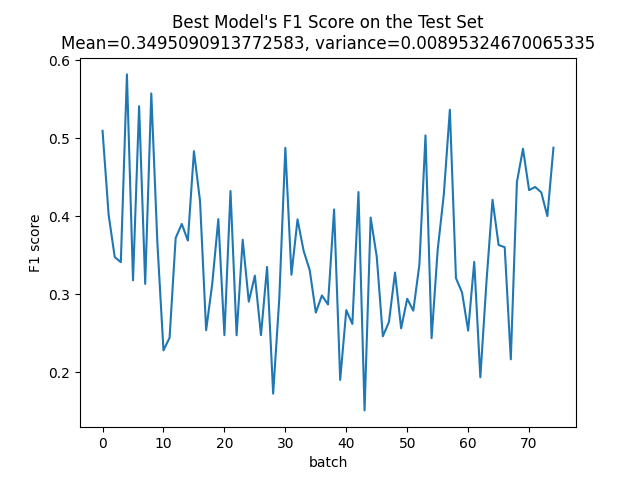
\includegraphics[width=0.65\textwidth,height=0.45\textwidth]{test.png}
\end{figure}
We observe that the generalization ability of the model is quite strong, in that the 
f1 score on the test set is close to that on the evaluation set. 
However, the model cannot yield an F1 score higher than 40\% on the test set or the evaluation set. 

\paragraph*{Remaining Problems}
Although the training and evaluation curves seems natural, the F1 scores on 
the evaluation set are all below 0.4, which is very low. 
We cannot trust this model even if it is the best model obtained.
We must try to improve the F1 score. 

\section{Initiative for Improvement}

\begin{itemize}
    \item Better loss function: Week 12-13. 
    We will try to use loss functions other than the Cross Entropy Loss to pay specail attention on an unbalanced dataset. 
    For example we may try to use focal loss functions and compare the results.     
    \item Better representation and architecture:  Week 12-13. 
    We plan to draw inspiration from state-of-the-art computer vision models designs to enhance the representation and generalization 
    ability of our model. For example, we might switch to using Visual Transformer, Detection Transformer and other architectures. 
    We can also try to optimize the design of the U net to adapt to the small-scale dataset. 
    \item Data augmentation: Week 14-15. 
    a. Synthesize more data. We can train a diffusion model on our train set and generate new data for training to increase the volume and diversity of the data set, in the hope that 
    we can improve the generalizability.   
    b. Enhance the quality of the data. We also play to adopt classical image augmentation techniques, like increasing the contrast 
    and rotating the image to discourage overfitting.
\end{itemize}



\bibliography{ref}
\bibliographystyle{plain}


%%%%%%%%%%%%%%%%%%%%%%%%%%%%%%%%%%%%%%%%%%%%%%%%%%%%%%%%%%%%%%%%%%%%%%%%%%%%%%%
%%%%%%%%%%%%%%%%%%%%%%%%%%%%%%%%%%%%%%%%%%%%%%%%%%%%%%%%%%%%%%%%%%%%%%%%%%%%%%%
% APPENDIX
%%%%%%%%%%%%%%%%%%%%%%%%%%%%%%%%%%%%%%%%%%%%%%%%%%%%%%%%%%%%%%%%%%%%%%%%%%%%%%%
%%%%%%%%%%%%%%%%%%%%%%%%%%%%%%%%%%%%%%%%%%%%%%%%%%%%%%%%%%%%%%%%%%%%%%%%%%%%%%%
\newpage
\onecolumn




\end{document}